\mode*

\section{Funktioner}

\subsection{Vad är bra med funktioner?}

\begin{frame}[fragile]
  \begin{block}{Funktioner}
    \begin{itemize}
      \item Som \enquote{miniprogram} som går att återanvända.
      \item Gör att vi kan minimera kodupprepningar.
      \item Ger färre problem, underlättar underhåll och utbyggnad.
    \end{itemize}
  \end{block}
\end{frame}

\begin{frame}[fragile]
  \begin{example}[Summera]
    \begin{lstlisting}
l = [1, 2, 3, 4]
print(sum(l))
    \end{lstlisting}
  \end{example}

  \begin{example}[Konkatenera]
    \begin{lstlisting}
l = ["flag", "pole", "polishing"]
print(sum(l))
    \end{lstlisting}
  \end{example}
\end{frame}

\begin{frame}[fragile]
  \begin{example}[Summera själv]
    \begin{lstlisting}
summa = 0

for i in lst:
  summa += i
    \end{lstlisting}
  \end{example}
\end{frame}


\subsection{Egna funktioner}

\begin{frame}[fragile]
  \begin{lstlisting}[basicstyle=\huge,numbers=none]
def func(parameters):
  # use {parameters}
  return results
  \end{lstlisting}
\end{frame}

\begin{frame}[fragile]
  \begin{example}[summera.py]
    \lstinputlisting{examples/summera.py}
  \end{example}
\end{frame}

\begin{frame}[fragile]
  \begin{example}[input-int.py]
    \lstinputlisting{examples/input-int.py}
  \end{example}
\end{frame}

\begin{frame}[fragile]
  \begin{example}[input-int-default.py]
    \lstinputlisting{examples/input-int-default.py}
  \end{example}
\end{frame}

\begin{frame}[fragile]
  \begin{example}[input-type.py, del 1]
    \lstinputlisting[linerange=3-12,firstnumber=3]{examples/input-type.py}
  \end{example}
\end{frame}

\begin{frame}[fragile]
  \begin{example}[input-type.py, del 2]
    \lstinputlisting[firstline=14,firstnumber=14]{examples/input-type.py}
  \end{example}
\end{frame}


\section{Inbyggda funktioner}

\begin{frame}
  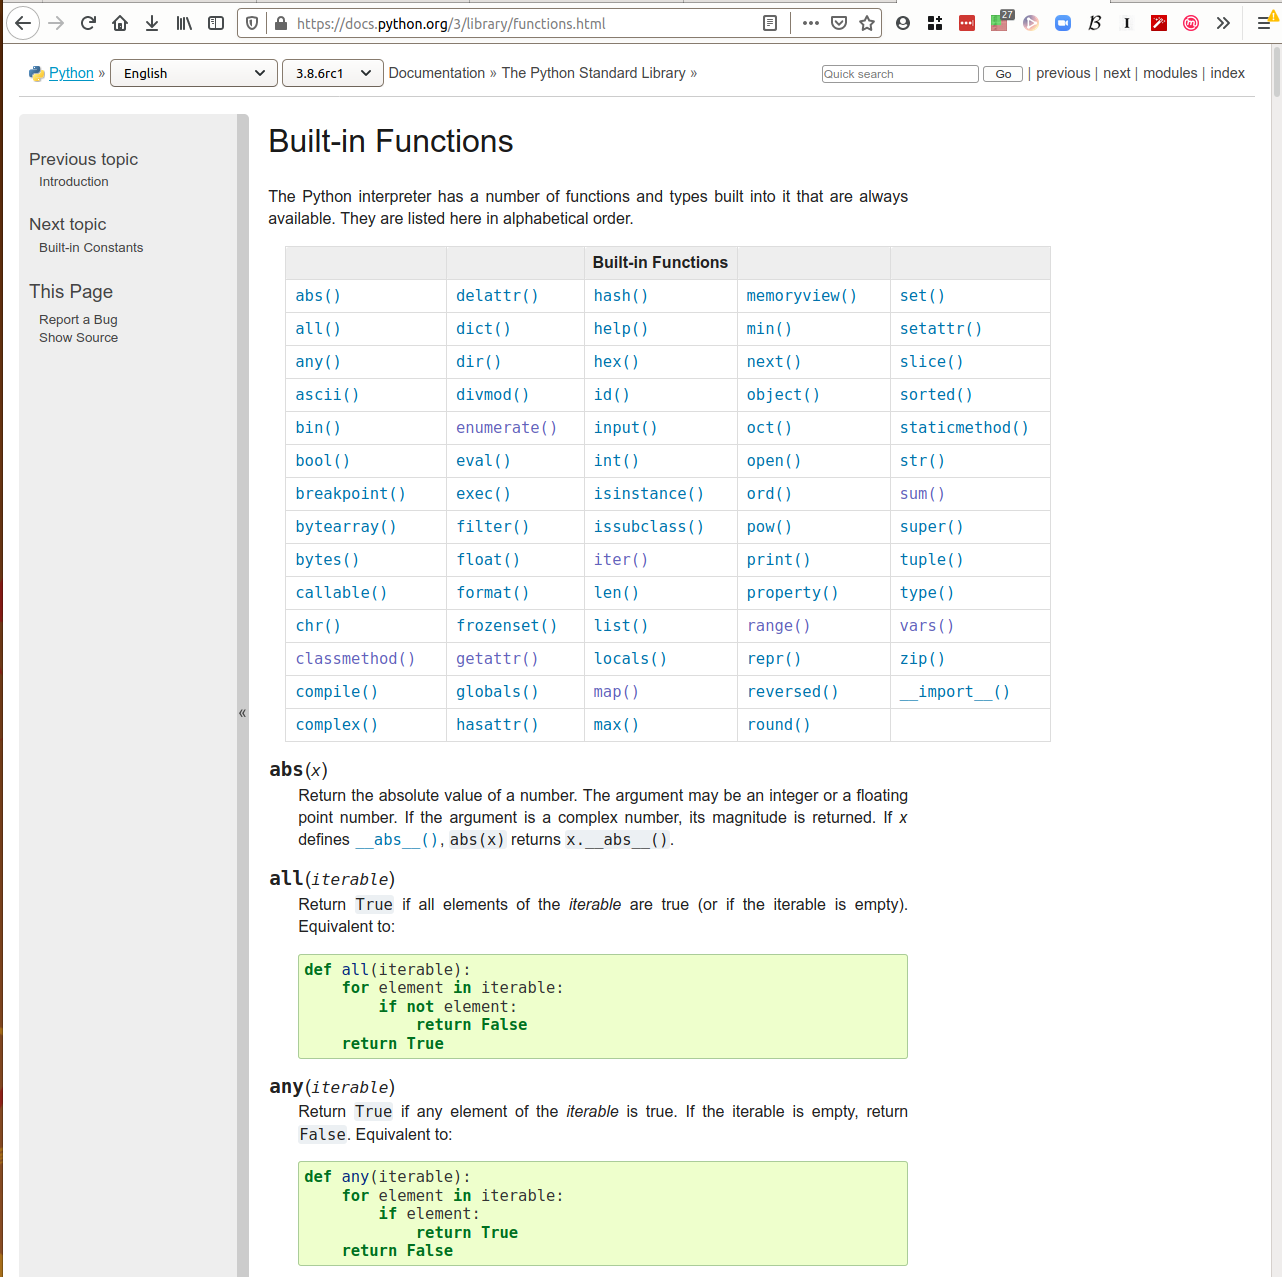
\includegraphics[width=\columnwidth]{figs/docs-built-in.png}
\end{frame}

\subsection{map() och filter()}

\begin{frame}[fragile]
  \begin{example}[mapping.py, del 1]
    \lstinputlisting[linerange=3-15,firstnumber=3]{examples/mapping.py}
  \end{example}
\end{frame}

\begin{frame}[fragile]
  \begin{example}[mapping.py, del 2]
    \lstinputlisting[firstline=16,firstnumber=17]{examples/mapping.py}
  \end{example}
\end{frame}

\begin{frame}[fragile]
  \begin{example}[filtering.py, del 1]
    \lstinputlisting[linerange=3-15,firstnumber=3]{examples/filtering.py}
  \end{example}
\end{frame}

\begin{frame}[fragile]
  \begin{example}[filtering.py, del 2]
    \lstinputlisting[firstline=21,firstnumber=21]{examples/filtering.py}
  \end{example}
\end{frame}

\subsection{Namnlösa (lambda-)funktioner}

\begin{frame}[fragile]
  \begin{example}[filter-lambda.py]
    \lstinputlisting{examples/filter-lambda.py}
  \end{example}
\end{frame}

\begin{frame}[fragile]
  \begin{example}[any-all.py, del 1]
    \lstinputlisting[linerange=7-18,firstnumber=7]{examples/any-all.py}
  \end{example}
\end{frame}

\begin{frame}[fragile]
  \begin{example}[any-all.py, del 2]
    \lstinputlisting[firstline=20,firstnumber=20]{examples/any-all.py}
  \end{example}
\end{frame}

\subsection{zip() och enumerate()}

\begin{frame}[fragile]
  \begin{example}[enum.py]
    \lstinputlisting{examples/enum.py}
  \end{example}
\end{frame}

\begin{frame}[fragile]
  \begin{example}[zip.py]
    \lstinputlisting{examples/zip.py}
  \end{example}
\end{frame}

